%!TEX root = ../main.tex

\chapter{基于有效字符的Web内容抽取}

\section{概述}
\label{sec:cevc-intro}
在Internet时代,Web新闻和博客都是很有代表性的信息发布和获取渠道。

Web新闻区别于传统的报纸,在互联网上发布意味着它能够触及更广大的受众,扩大自己的影响力,
对热点新闻的实时推送也提高了信息传播的即时性。
阅读Web新闻了解实事动态已经成为广大网民的生活习惯,很多传统媒体也纷纷推出了自己的Web新闻。

博客(blog,weblog的缩写,也叫网络日志)是发布在互联网上的文章集合,通常由个人撰写和管理。
博客给普通大众提供了一个表达自己观点和态度的平台,人们还能在文章后发表评论,
形成一个庞大的社区,促进信息的交流。

但除了新闻正文之外,一个典型的新闻网页还包含导航栏、广告、推荐链接和版权信息等,
这些与正文无关的额外内容,通常称为噪声。
Gibson在2005年的研究\cite{gibson2005volume}显示,
网页模板在整个网页中占据了$40\%$--$50\%$的字节量,而且这个比例正以每年$6\%$的速度增长。
以一篇新浪新闻\footnote{http://news.sina.com.cn}为例,如图~\ref{fig:news}~所示,
红色实线圈出的内容都与正文无关,它们占据了网页一半以上的篇幅。

博客和新闻类似,都属于正文集中的网站,博客网页的噪声主要有导航栏、广告和博客相关文章等。
以一篇网易博客\footnote{http://blog.163.com}为例,如图~\ref{fig:blog}~所示,
红色实线圈出的是与正文无关的内容。

\begin{figure}[htbp]
\centering
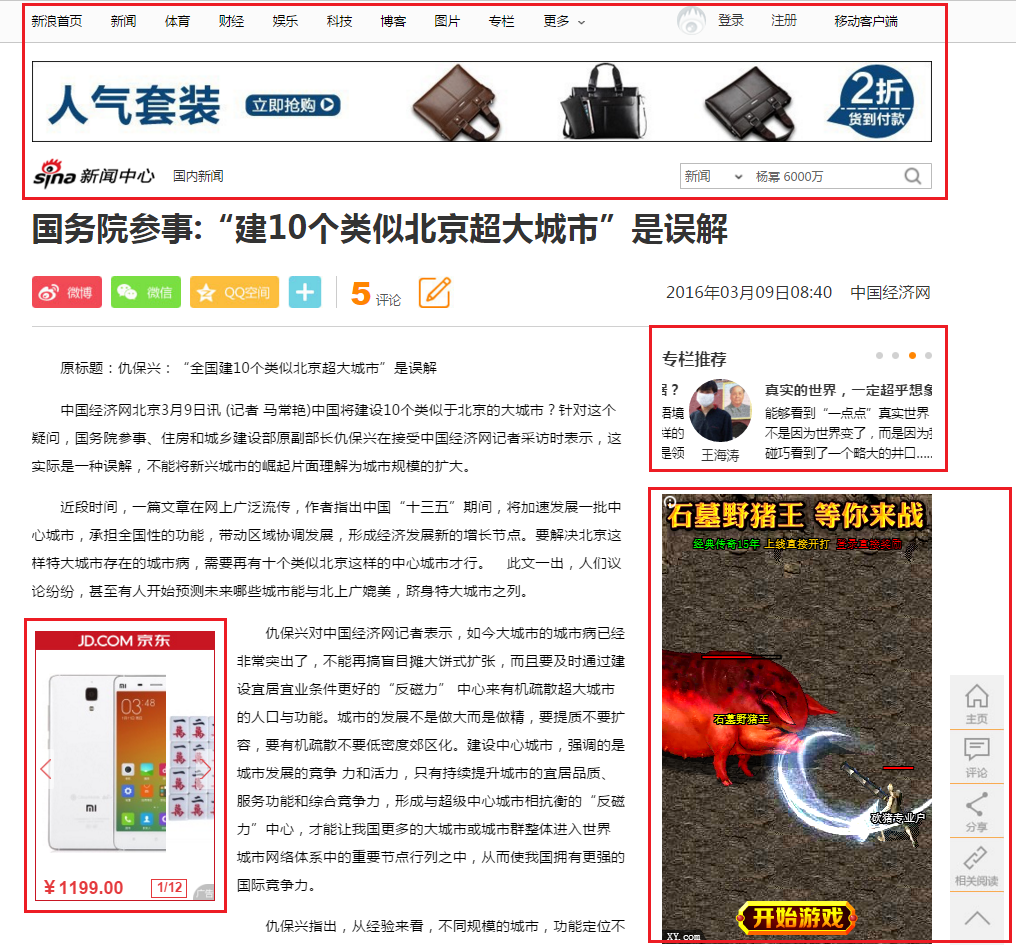
\includegraphics[width=0.9\textwidth,height=0.45\textheight]{news}
\caption{新浪新闻实例}
\label{fig:news}
\end{figure}

\begin{figure}[htbp]
\centering
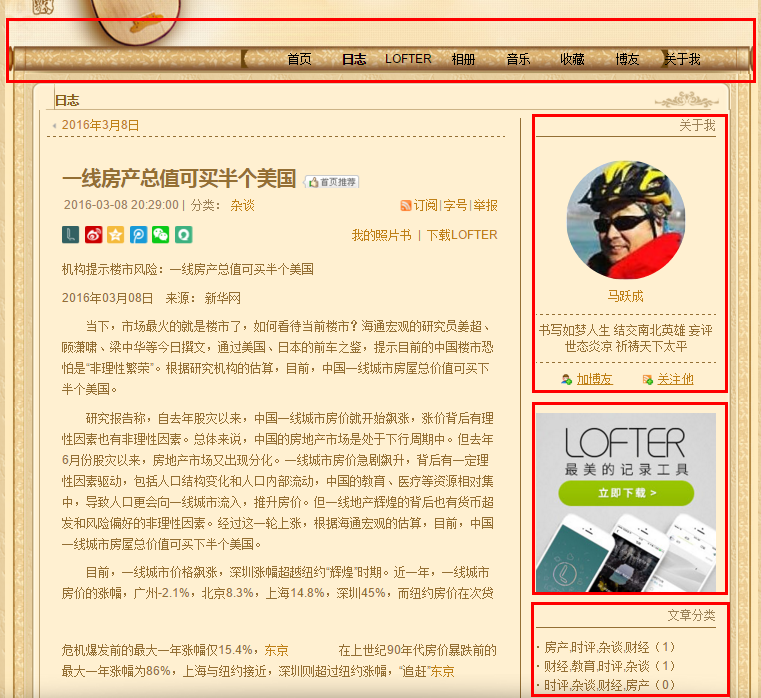
\includegraphics[width=0.9\textwidth,height=0.45\textheight]{blog}
\caption{网易博客实例}
\label{fig:blog}
\end{figure}

从网页中抽取核心内容,过滤这些噪声,不仅能够给用户提供“干净”的内容,
也能节约爬虫系统的存储开销,减小索引规模,提升后续自然语言处理的效果。
由于新闻和博客网页布局与内容抽取目标的相似性,本章将两者合并处理,
提出一种基于有效字符的Web内容抽取方法,~\ref{sec:cevc-method}~节详述该方法
CEVC(Content Extraction via Valid Characters),
~\ref{sec:cevc-other}~节简单介绍对比算法CETR,CETD和CEPR并给出算法实现细节,
~\ref{sec:cevc-experiment}~节进行对比实验并分析结果。

\section{CEVC方法}
\label{sec:cevc-method}

\subsection{DOM}
\label{subsec:dom}
在网页内容抽取的研究工作中,为了利用HTML文档的结构信息,
很多方法都是在DOM的基础上进行\citeup{yi2003eliminating,sun2011dom,wu2013web}
这里对DOM做简单介绍。

DOM(Document Object Model,文档对象模型)是一个跨平台语言无关的规范,
用来表示和操作HTML,XHTML和XML的对象\footnote{http://www.w3.org/DOM/}。
每个文档所包含的节点被组织为一个树型结构,称为DOM树。
DOM树节点所表示的对象可以通过一组方法来寻址或操作,这些接口以API的形式描述。
通过这样一种规范,程序和脚本能够动态访问和更新文档的内容、结构以及风格,
文档经过后续处理后,还能将结果更新到展示的页面上。

上世纪90年代,网景公司和微软公司相继推出自己的浏览器,和浏览器端的脚本语言JavaScript。
JavaScript让Web开发者能够创造和用户交互的网页,检测用户产生的事件并更新HTML文档,
这类第一代的语言被称为Legacy DOM。
随后W3C(World Wide Web Consortium,万维网联盟)制定了第一版的DOM标准,
之后相继发布了新版本。
截止到2005年,W3C DOM中的大部分特性都能被主流浏览器广泛支持。

HTML文档可以解析为DOM树,每个HTML标签对应一个DOM树节点,
父子节点对应HTML标签的嵌套关系,兄弟节点对应HTML标签的并列关系,
这样就把序列化的HTML文档转换为层次化的对象模型,便于程序的访问和操作。

\begin{figure}[htbp]
\begin{example}
\label{ex:html}
一个简化的HTML代码片段
\end{example}
\begin{verbatim}
 1. <html>
 2.   <head> ... </head>
 3.   <body>
 4.     <div class="nav-wrap">
 5.       <h1>Small Vintage Plane Crashes in Hudson River</h1>
 6.     </div>
 7.     <div> ... </div>
 8.     <div class="ep-content">
 9.       <a>
10.         <span>From Stefan Holt</span>
11.       </a>
12.       <p>The plane was on a photo flight with two other planes ...</p>
13.       <p>They say they saw the pilot try to get out but ...</p>
14.     </div>
15.   </body>
16. </html>
\end{verbatim}
\end{figure}

\begin{figure}[htbp]
\centering
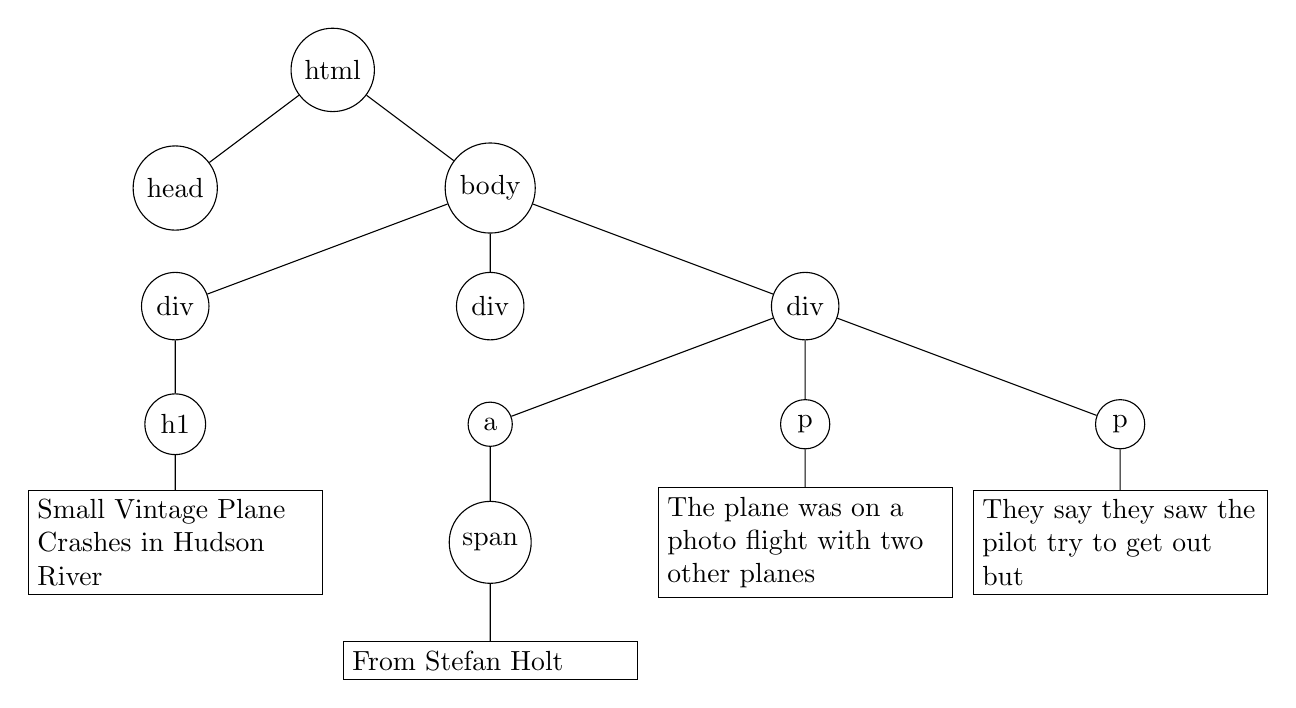
\begin{tikzpicture}[
sibling distance=4cm,
tag/.style={circle, draw},
leaf/.style={rectangle, draw, text width=3.5cm}
]
\node[tag]{html}
  child{node[tag]{head}}
  child{node[tag]{body}
    child{node[tag]{div}
      child{node[tag]{h1}
        child{node[leaf]{Small Vintage Plane Crashes in Hudson River}}
      }
    }
    child{node[tag]{div}}
    child{node[tag]{div}
      child{node[tag]{a}
        child{node[tag]{span}
          child{node[leaf]{From Stefan Holt}}
        }
      }
      child{node[tag]{p}
        child{node[leaf]{The plane was on a photo flight with two other planes}}
      }
      child{node[tag]{p}
        child{node[leaf]{They say they saw the pilot try to get out but}}
      }
    }
  }
;
\end{tikzpicture}
\caption{一个简化的DOM树}
\label{fig:dom}
\end{figure}

例~\ref{ex:html}~所示的HTML片段经过解析后形成一个DOM树,如图~\ref{fig:dom}~所示。
每个HTML标签都与一个DOM树节点对应,HTML标签的属性仍然附属在DOM节点上。
网页中能够显示的具体文本都位于DOM树的叶节点上,DOM树的内部节点只负责结构控制和布局。
HTML的根节点是\texttt{<html>},一般包含两个节点\texttt{<head>}和\texttt{<body>}。
网页的可视区域都从\texttt{<body>}标签开始,
因此我们的研究对象是\texttt{<body>}标签下的内容。

\subsection{有效字符}
回顾图~\ref{fig:news}~和~\ref{fig:blog}~,我们注意到网页正文一般是文本密集的区域,
而噪声信息则包含高度格式化的、简短的文本。
通过大量实例分析,我们发现噪声信息通常包含链接,无论是导航栏的网站板块链接,
还是广告链接或相关文章链接,它们都符合这个特点,吸引用户点击来完成自己的职能。
反之,一段不包含链接的文本更有可能是网页核心内容。

链接在HTML文档中由\texttt{<a>}标签组成,a代表anchor,所以链接内的文本也称为锚文本。
DOM节点的继承关系使得包裹在\texttt{<a>}标签内的所有文本都变成锚文本,
例如图~\ref{fig:dom}~中的\texttt{From WWW}虽然在\texttt{<span>}下,
但其祖先节点是一个\texttt{<a>}标签,因此也变成了锚文本。

除此之外,噪声信息较为简短,甚至不能组成一个语义完整的句子,我们可以利用停止词来刻画这一特征。
停止词是自然语言处理中过滤掉的词\footnote{https://en.wikipedia.org/wiki/Stop\_words},
它们在一篇文章中大量出现,多为冠词、介词或连词,却对文章主体内容贡献很小。
尽管停止词对文章没有多大意义,但一段话如果没有停止词,那么它就不是一个语义完整的句子,
更有可能是一组关键词的堆砌,而不是网页的核心内容。
例~\ref{ex:stopwords}~节选自网页中的一段话,以下划线的形式标注了其中的停止词,
可见停止词在正文中是普遍存在的。

\begin{figure}[htbp]
\begin{example}
\label{ex:stopwords}
网页中的停止词示例
\end{example}
买房\underline{还是}租房?
\underline{这是}眼下很多\underline{人}要面对\underline{的}一道选择题。
如果简单比较,一边\underline{是}数额很大\underline{的}买房负担,
一边\underline{是}相对\underline{可}接受\underline{的}租金价格,
似乎租房应更受欢迎,现实\underline{却}非如此。
山东某县一位购房者对笔者道出心声:“买房子,政府一平方米补贴100元,一套房子能省1万多元。
租房子,\underline{啥}实惠没有,\underline{还}总\underline{被}赶来赶去,
住\underline{着不}踏实。”
\underline{他}最终\underline{还是}选择\underline{了}勒紧裤腰带贷款买房。
\end{figure}

结合上述链接和停止词与网页噪声的相关性,我们提出一个有效字符的概念:

\begin{definition}
\label{def:validchar}
$i$是DOM中的一个叶节点,如果$\forall p \in ancestors(i)$都有$tag(p) \neq a$,
并且$stopwords(i) > 0$,那么$i$所包含的文本就是有效字符。
\end{definition}

定义~\ref{def:validchar}~中,$ancestors(i)$表示$i$的所有祖先节点,
$tag(p)$表示$p$的标签名,$stopwords(i)$表示$i$的停止词个数。
有效字符代表网页中那些更有可能是正文的文本,忽略了链接噪声和太过松散的短语,
有效字符越多,代表这个节点更有可能是正文。

为了利用DOM节点的有效字符分布信息,我们需要计算每个DOM节点下所包含的有效字符个数,
可以将其作为一项属性,插入到DOM节点中,便于后续的处理。
在计算之前,首先去除网页中的\texttt{<script>},\texttt{<style>}和\texttt{comment}。
这些脚本、样式文件和注释对网页显示的文本内容没有贡献,却可能干扰计算结果。

如算法~\ref{algo:cevc-count}~所示,这是一个自顶向下的递归计算过程。
ValidChars被作为属性,存储在节点中。
当前节点有子节点时,递归计算子节点,然后当前节点的有效字符数被累加到父节点上。
当前节点是叶节点时,根据定义~\ref{def:validchar}~判断它包含的文本是否是有效字符,
如果是,则将非空白字符数累加到父节点上。
这里忽略了空白字符,是为了排除网页排版风格带来的影响,让计算结果更加稳定。

算法~\ref{algo:cevc-count}~的主要操作就是遍历DOM树,
所以它的运行时间与DOM树中的节点数成正比,时间复杂度为$O(n)$,$n$是DOM树中的节点数。
为了在内存中存储解析后的DOM树,其空间复杂度也是$O(n)$。

\begin{algorithm}[htbp]
\caption{countValidChars(N)}
\label{algo:cevc-count}
\KwIn{DOM node N}
\KwOut{DOM node N}

\eIf{N has child nodes} {
  \For{C $\in$ N.children()}{
    countValidChars(C) \;
  }
  N.parent.validChars += N.validChars \;
}{
  \tcp{N is a leaf text node}
  \If{N consists of valid characters}{
    length = getNonSpaceLength(N) \;
    N.parent.validChars += length \;
  }
}
\end{algorithm}

经过算法~\ref{algo:cevc-count}~的处理,
我们可以得到一个标注了各个节点ValidChars的HTML页面,如图~\ref{fig:news-stepinto}~所示。

\begin{figure}[t]
\centering
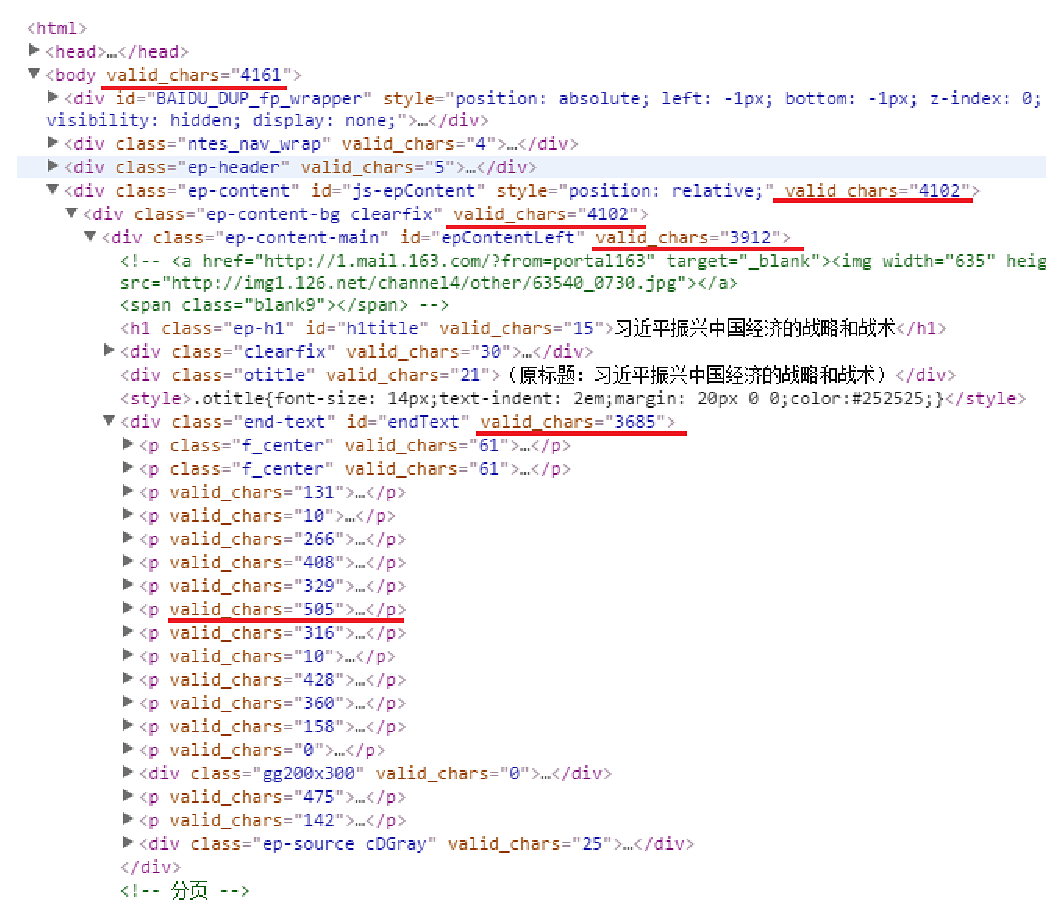
\includegraphics[width=0.9\textwidth]{news-stepinto}
\caption{有效字符示例}
\label{fig:news-stepinto}
\end{figure}

\subsection{定位核心内容块}
经过大量实例分析,我们发现对于新闻、博客这类正文信息集中的网站,
核心内容块都位于同一个父节点之下,通常表现为文本的段落。
图~\ref{fig:news-stepinto}~中的新闻正文位于\texttt{<div\#endText>}节点之下,
是由\texttt{<p>}标签构成的段落。

这里\texttt{div\#endText}的记号是CSS选择符,可以指定CSS样式规则作用在哪些DOM节点上,
简单的用法是\texttt{div\#endText}选择\texttt{<div id='endText'>}这样的标签,
而\texttt{div.text}选择\texttt{<div class='text'>}这样的标签。
和正则表达式、XPath一样,CSS选择符也可以用来在HTML文档中描述提取规则。

现在我们看到每个DOM节点上都标注了有效字符的个数,有效字符越多表明这个节点越可能是核心内容。
但这个比较必须在同一个层次的兄弟节点间才有意义,因为有效字符数是嵌套包含的,
毫无疑问\texttt{<body>}的有效字符数最多。
如果从\texttt{<body>}节点开始,每次都选择有效字符数最多的子节点深入,
就能定位出一条从\texttt{<body>}通往核心内容块的正确路径,
如图~\ref{fig:news-stepinto}~中红线标示的节点。

每次沿着有效字符数最大的子节点不断深入,意味着我们每一步放弃了信息量较小的兄弟节点。
这个过程不能一直持续下去,否则会陷入到叶节点中,而错失最终的父节点。
如图~\ref{fig:news-stepinto}~所示,最后一步进入了一个\texttt{<p>}标签,
而错失了真正的核心内容块\texttt{<div\#endText>}。
我们需要定义一个指标,来判断何时停止向下深入的过程。

\begin{definition}
\label{def:mcr}
$i$是DOM树中的一个节点,$i$的最大子节点字符占比MCR(Max Chars Ratio)如下所示,
其中$C_i$表示$i$的有效字符数,$j$是$i$的子节点:
\begin{equation}
MCR_i = max_{j \in children(i)} \frac{C_j}{C_i}
\end{equation}
\end{definition}

在DOM树中每次向下深入一步,我们认为最大子节点包含了父节点的绝大部分文本信息。
当定义~\ref{def:mcr}~中的MCR低于一个阈值时,
表明最大子节点的有效字符数并不足以在父节点中占据统治地位,
即最大子节点的文本不能在可接受的损失范围内代表父节点,这时候放弃兄弟节点是不合理的,
因此向下深入的过程应立即终止,当前节点就是核心内容块。

\begin{figure}[htbp]
\begin{example}
\label{ex:mcr}
MCR计算过程
\end{example}
\begin{verbatim}
1. <body> valid_chars=4161 MCR=0.99
2. <div#js-epContent> valid_chars=4102 MCR=1.0
3. <div.ep-content-bg> valid_chars=4102 MCR=0.95
4. <div#epContentLeft> valid_chars=3912 MCR=0.94
5. <div#endText> valid_chars=3685 MCR=0.14 核心内容块
6. <p> valid_chars=505
\end{verbatim}
\end{figure}

如例~\ref{ex:mcr}~所示,每一行显示的都是图~\ref{fig:news-stepinto}~中各层的最大子节点。
在到达\texttt{<body\#endText>}之前,MCR一直保持$0.9$以上的高比率,
而\texttt{<body\#endText>}的MCR锐减到$0.14$,因为此时已深入到正文的一个段落中,
这个段落无法代表正文的内容,\texttt{<body\#endText>}就是最终的核心内容块。

上述过程如算法~\ref{algo:cevc-stepinto}~所示。
在经过算法~\ref{algo:cevc-stepinto}~\texttt{countValidChars}预处理后的DOM树上,
先遍历子节点,找出有效字符数最大的子节点,并累加所有字符数。
然后选定最大子节点\texttt{maxNode},如果MCR小于一个阈值$\alpha$就停止并输出当前节点,
否则在MaxNode上继续递归调用算法\texttt{stepInto}。
\texttt{output}过程负责把当前节点的所有有效字符输出,作为核心内容抽取的结果返回。
注意第~\ref{algo:line:edge}~行,当遇到一种极端情况,正文仅仅包含一个段落,
那么StepInto深入到最底层仍然会有很高的MCR,导致无法终止直到进入叶节点。
这时候采取一种简单的策略,认为当前节点的父节点就是核心内容块。
后续实验表明,这是一个简单也可以接受的方案。

通过在DOM树中不断选择最有代表性的子节点不断深入,
算法~\ref{algo:cevc-stepinto}~至多被递归调用$h$次,
$h$是DOM树的高度,所以其时间复杂度为$O(h)$,能够很快运行结束。

\begin{algorithm}[htbp]
\caption{stepInto(N)}
\label{algo:cevc-stepinto}
\KwIn{DOM node N}
\KwOut{main content}

maxNode = null \;
maxValidChars = 0 \;
totalValidChars = 0 \;
\For{$C \in N.children()$}{
  totalValidChars += C.validChars \;
  \If{$C.validChars > maxValidChars$}{
    maxValidChars = C.validChars \;
    maxNode = C \;
  }
}

\eIf{maxNode is not null}{
  MCR = maxValidChars / totalValidChars \;
  \eIf{$MCR < \alpha$}{
    \Return output(N) \;
  }{
    stepInto(maxNode) \;
  }
}{
  \tcp{Step into the leaf node}
  \Return output(N.parent) \; \label{algo:line:edge}
}
\end{algorithm}

\subsection{算法实现}
本文中CEVC算法使用Python 2.7实现。

面对HTML网页中普遍存在的代码错误,例如缺失结束标签、使用非标准的标签和错误的嵌套等,
这里使用Python第三方库
BeautifulSoup\footnote{http://www.crummy.com/software/BeautifulSoup/}
来尽可能纠正这些错误。
BeautifulSoup是一个可以从HTML或XML文件中提取数据的Python库,
它为操作DOM提供了一套方便的接口,底层调用lxml等具体的解析器,
能够处理有代码错误的网页。

CEVC算法中需要识别停止词,这里使用了
jieba\footnote{https://github.com/fxsjy/jieba}中的停止词模块。
jieba(结巴中文分词)是一个开源的Python中文分词组件,MIT协议授权,
支持多种分词模式。

\section{对比算法及实现}
\label{sec:cevc-other}

\subsection{CETR}
Weninger等人于2010年提出CETR(Content Extraction via Tag Ratios)算法
\citeup{weninger2010cetr}。

CETR的基本概念是定义了Tag Ratio。
它以“行”为单位读取HTML网页并处理,分别计算每一行的Tag Ratio,
即非HTML标签字符个数与HTML标签个数的比值。
如果遇到HTML标签个数为零的特殊情况,该行的Tag Ratio就是所有字符的个数。
作者认为Tag Ratio越高,反映了文本密集程度越高,更有可能是网页的核心内容。

通过计算可以得到每一行Tag Ratio的直方图,最直接的方法就是找到一个阈值,
所有Tag Ratio高于此阈值的行被认为是有效内容,
所有Tag Ratio低于此阈值的行被认为是噪声内容。
如何找到这样一个合适的阈值,就成为了文章的主要研究内容。

为了提升直方图的区分度,作者对数据进行了高斯平滑。
标准的高斯平滑算法主要用来做图像处理,是应对连续数据的,作者重新实现为一维的离散操作。
公式(~\ref{eq:cetr-kernel}~)是高斯核函数的构造过程,
给定窗口大小为$2(\lceil \sigma \rceil) + 1$。

\begin{equation}
\label{eq:cetr-kernel}
k_i = \sum_{j=-\lceil \sigma \rceil}^{\lceil \sigma \rceil}
e^{\frac{-j^2}{2\sigma^2}}, 0 \leq i \leq 2(\lceil \sigma \rceil)
\end{equation}

公式(~\ref{eq:cetr-kernel2}~)中高斯核函数$k$被处理为$k'$。

\begin{equation}
\label{eq:cetr-kernel2}
k_i' = \frac{k_i}{\sum_{j=0}^{\lceil \sigma \rceil}k_j},
\lceil \sigma \rceil \leq i \leq 2(\lceil \sigma \rceil)
\end{equation}

最后高斯核函数$k'$和直方图$T$一起做卷积运算,形成平滑后的直方图$T'$,
如公式(~\ref{eq:cetr-kernel3}~)所示。

\begin{equation}
\label{eq:cetr-kernel3}
T_i' = \sum_{j=-\lceil \sigma \rceil}^{\lceil \sigma \rceil}
k'_{j+\lceil \sigma \rceil} T_{i-j},
\lceil \sigma \rceil \leq i \leq len(T)-\lceil \sigma \rceil
\end{equation}

上述以阈值划分直方图的方法,其缺陷是将Tag Ratio仅仅视为一组数据,
而不是有序的序列,为了利用有序的信息,作者提出了一个二维模型。

\begin{equation}
\label{eq:cetr-kernel4}
f'(T_i')=G_i=\frac{\sum_{j=0}^{\alpha} T_{i+j}'}{\alpha} - T_i',
0 \leq i < len(T') - \alpha
\end{equation}

注意到$len(G) \neq len(T')$,实际上$len(G)=len(T')-1$
因为$G$是一组数据的差异值。
接着使用公式(~\ref{eq:cetr-kernel3}~)平滑$G$得到$G'$。
最后计算$\hat{G}$使得$\hat{G_i}=\vert G_i' \vert$,对于$G'$中的每一个$i$。

将平滑后的Tag Ratio $T'$和$T'$的Absolute Smoothed Derivatives $\hat{G}$
联合组成二维模型,相比于一维数据,更加具有区分度。

随后作者使用K-means聚类算法,将所有的样本点进行聚类,这里使用$k=3$。
与一般的K-means聚类不同,将其中一个簇的中心点固定为二维坐标系的原点,
这样可以使得剩余簇远离原点,并且很容易划分最终的结果,
即中心点固定在原点的簇是噪声内容,而剩余簇代表有效内容。

\textbf{实现细节}

作者一共提出了三种算法,记为CETR-TM、CETR-KM和CETR。
CETR-TM是阈值算法,CETR-KM是一维数据上的K-means聚类算法,
CETR是二维数据上的K-means聚类算法。
根据作者的实验对比,CETR的抽取性能最佳,也是本章中参与对比的算法。

作者提供了Java实现的算法源代码\footnote{http://www3.nd.edu/~tweninge/cetr/},
我们对其进行了简单的包装,以Python接口调用并参与后续的评价指标计算。

\subsection{CETD}
Sun等人于2011年提出CETD(Content Extraction via Text Density)算法
\citeup{sun2011dom}。

CETD算法的核心概念是Text Density,它在DOM树的基础上定义,
而不像CETR那样以行为单位处理,更能利用HTML的结构信息。
Text Density的基础定义如~\ref{def:cetd-td}~所示。

\begin{definition}
\label{def:cetd-td}
如果$i$是一个标签(对应DOM树中的一个节点),那么$i$的Text Density($TD_i$)
是其字符个数和标签个数的比值:
\begin{equation}
TD_i = \frac{C_i}{T_i}
\end{equation}
\end{definition}

在进一步研究后,作者发现很多网页噪声由超链接组成,基于这样的观察,
对每个节点计算了两个额外的统计指标:
\begin{enumerate}
\item \textit{LinkCharNumber}:子树中所有链接字符的个数
\item \textit{LinkTagNumber}:子树中所有链接标签的个数
\end{enumerate}

在加入了链接的统计信息后,定义了Composite Text Density:

\begin{definition}
\label{def:cetd-ctd}
如果$i$是一个标签(对应DOM树中的一个节点),
那么$i$的Composite Text Density($CTD_i$)是:
\begin{equation}
CTD_i = \frac{C_i}{T_i}\log_{ln(\frac{C_i}{\neg LC_i}LC_i + 
\frac{LC_b}{C_b}C_i + e)}(\frac{C_i}{LC_i}\frac{T_i}{LT_i})
\end{equation}
\end{definition}

定义~\ref{def:cetd-ctd}~中,$C_i$表示$i$节点下的所有字符个数,
$T_i$表示$i$节点下的所有标签个数,$LC_i$表示链接字符个数,
$\neg LC_i$表示非链接字符个数,$LT_i$表示链接标签个数,
$LC_b$表示\texttt{<body>}节点下的所有链接字符个数,
$C_b$表示\texttt{<body>}节点下的所有字符个数。
遇到分母为零的情况,直接将分母设为1。

为了从Text Density中区分噪音节点和内容节点,
最直接的方法是以\texttt{<body>}的Text Density作为划分阈值。
因为\texttt{<body>}比噪音节点包含更多的文本内容,
又比内容节点包含更多的超链接,所以它是一个足够区分二者的中间值。

数据平滑可以削峰填谷,增加区域内部的内聚性和区域之间的差异性,
虽然一般来说数据平滑可以取得较好的结果,它仍然会丢失一些低文本密度的节点。
为了改进传统的平滑、基于阈值划分的方法,作者提出了DensitySum的方法。

DensitySum基于这样的观察,网页的内容块在DOM树结构中都属于一个祖先节点,
并且内容节点的文本密度显著高于噪声节点。
如果把一个节点的所有子节点的文本密度累加,称为DensitySum,
那么DensitySum就会在内容节点上取得一个极高值。
其定义如下:

\begin{definition}
\label{def:cetd-densitysum}
如果$N$是一个标签(对应DOM树中的一个节点),$i$是$N$的一个子节点,
那么$N$的DensitySum就是它所有子节点文本密度之和:
\begin{equation}
DensitySum_N = \sum_{i \in C} TextDensity_i
\end{equation}
\end{definition}

\textbf{实现细节}

作者一共提出了三种算法CETD-DS,CECTD-S和CECTD-DS。
CETD-DS是基于Text Density和DensitySum的算法,
CECTD-S是基于Composite Text Density和数据平滑的算法,
CECTD-DS是基于Composite Text Density和DensitySum的算法。
根据作者的实验对比,CECTD-DS的抽取性能最佳,也是本章中参与对比的算法。
如无特殊说明,以后简称CECTD-DS为CETD算法。

根据\cite{sun2011dom}给出的算法伪代码,我们用Python 2.7重新实现了CETD。
为了处理HTML文档中的错误,同样使用了BeautifulSoup尽可能纠正。
并通过BeautifulSoup,将HTML文档转化为内存中的DOM树,
在进行计算和操作之前去除了所有\texttt{<script>},\texttt{<style>}和\texttt{comment}。

\subsection{CEPR}
Wu等人于2013年提出了CEPR(Content Extraction via Path Ratios)算法
\citeup{wu2013web}。

CEPR算法的核心概念是\textbf{T}ext to Tag \textbf{P}ath \textbf{R}atio,或简称为TPR。
作者首先在DOM树的基础上,提出Tag Path的概念,
即从根节点到文本叶节点\footnote{文本全部分布在DOM树的叶节点上,见~\ref{subsec:dom}~节}
的一条路径,由HTML标签构成。
例如\texttt{div.div.div.h1}就是一条Tag Path。
在Tag Path的基础上,提出Text to Tag Path Ratio:

\begin{definition}
\label{def:cepr-tpr}
假设$p$是一条Tag Path,那么$p$的Text to Tag Path Ratio(TPR)就是:
\begin{equation}
TPR(p) = \frac{\sum_{v \in accNodes(p)}length(c(v))}{\vert accNodes(p) \vert}
\end{equation}
\end{definition}

定义~\ref{def:cepr-tpr}~中,$accNodes(p)$是路径$p$能够访问的文本叶节点集合,
$c(v)$是文本叶节点$v$的文本内容。
TPR既是每条Tag Path的度量值,也是每个文本叶节点的度量值。
在一般网页上,通常有这样的观察:
\begin{enumerate}
\item 内容节点通常有相似的Tag Path,而噪声节点也有相似的Tag Path;
\item 内容节点通常包含更多的文本,而噪声节点通常包含较少的文本;
\item 所有文本节点都是叶节点。
\end{enumerate}
显然,内容节点的TPR值较高而噪声节点的TPR值较低,可以用来抽取核心内容。
TPR的阈值定为$\tau = \lambda \sigma(H')$,$\lambda$是调节参数,
$\sigma(H')$是直方图的标准差。

进一步的研究表明,网页内容会包含标点符号,而噪声则没有。
除此之外,文本长度和标点符号个数在内容节点中的分布差异很大,在噪声节点中却很少变化。
作者进一步提出了
\textbf{E}xtended \textbf{T}ext to Tag \textbf{P}ath \textbf{R}atio(ETPR):

\begin{definition}
\label{def:cepr-etpr}
假设$p$是一条Tag Path,那么$p$的Extended Text to Tag Path Ratio(ETPR)就是:
\begin{equation}
ETPR(p) = TPR(p) \cdot 
\frac{\sum_{v \in accNodes(p)}puncNum(c(v))}{\vert accNodes(p) \vert}
\cdot \sigma_{cs} \cdot \sigma_{ps}
\end{equation}
\end{definition}

定义~\ref{def:cepr-etpr}~中$puncNum(c(v))$是$v$中标点符号的个数,
$\sigma_cs$和$\sigma_ps$分别是路径$p$能访问的文本叶节点集合中
文本长度和标点符号个数的标准差。

在\cite{weninger2010cetr}的高斯平滑算法基础上,
作者提出以编辑距离作为权重,改善平滑效果。
即公式(~\ref{eq:cetr-kernel3}~)的卷积运算修改为公式(~\ref{eq:cepr-kernel}~)。

\begin{equation}
\label{eq:cepr-kernel}
H_i' = \sum_{j=-r}^{r} w_{ij} k_j' H_{i-j}, r \leq i \leq len(H)-r
\end{equation}

其中权重定义为:
\begin{equation}
\label{eq:cepr-w}
w_{ij} = 
\left\{\begin{matrix}
1, p_i = p_j \\ 
\frac{1}{(dist(p_i, p_j))^\alpha}, p_i \neq p_j
\end{matrix}\right.
\end{equation}

公式(~\ref{eq:cepr-w}~)中的$dist(p_i, p_j)$是路径$p_i$和$p_j$的
编辑距离\citeup{levenshtein1966binary},
$\alpha$是调节编辑距离对平滑贡献的参数。

\textbf{实现细节}

作者一共提出了三种算法CEPR-TPR,CEPR-ETRP和CEPR-SETPR。
CEPR-TPR是基于TPR的算法,CEPR-ETPR是基于扩展的ETPR的算法,
CEPR-SETPR是基于ETPR并进行加权高斯平滑处理后的算法。
根据作者的实验对比,CEPR-SETPR的抽取性能最佳,也是本章中参与对比的算法。
如无特殊说明,以后简称CEPR-SETPR为CEPR算法。

根据\cite{wu2013web}给出的算法伪代码,我们用Python 2.7重新实现了CEPR。
同样使用了BeautifulSoup来处理HTML文档,转化为DOM树结构。
CEPR算法需要判断标点符号,这里使用了Python标准库的\texttt{string.punctuation}
来定义英文标点符号,并补充了一个中文标点符号列表。
CEPR算法需要计算路径的编辑距离,这里以Tag的尺度计算,
而不是直接计算两个Tag Path字符串的编辑距离。

我们在小规模数据集上进行了参数调整实验,确定了和\cite{wu2013web}中一致的参数配置:
$\lambda=0.8$,$\alpha=1$和$r=1$。

\section{实验与分析}
\label{sec:cevc-experiment}

\subsection{评价指标}
为了验证算法的抽取效果,我们定义标准评价指标精确率Precision、召回率Recall和
F\textsubscript{1}。
通过比较算法抽取的文本$e$和金标准的文本$g$,Precision、Recall和
F\textsubscript{1}可以如下计算:

\begin{equation}
P = \frac{LCS(e,g).length}{e.length}, R = \frac{LCS(e,g).length}{g.length}
\end{equation}
\begin{equation}
F_1 = \frac{2 \times P \times R}{P + R}
\end{equation}

对于中文文档,视为字符的序列而不进行分词处理,
因为中文分词需要额外的依赖,而且CEVC算法重在对有效字符的统计而不需要词的信息。
$LCS(e,g)$是$e$和$g$的最长公共子序列,
文档中两个相同的字符如果位置顺序不同,也会被LCS的计算区分开来。
相比于\cite{weninger2010cetr}中使用的计算方法,把两个文档的词视为两个集合,
该方法利用了不同词的位置信息而更加准确。

除了标准评价指标外,这里给出另一个常用的评价方法Score。
Score在\cite{sun2011dom}和\cite{wu2013web}中都提到过,
是为了替换CleanEval中运算开销很大的
Levenshtein Distance\citeup{levenshtein1966binary}
(对齐两个字符串所需要的插入、删除操作次数,不允许替换),
而使用最长公共子序列计算产生的。
其定义如下:

\begin{equation}
Score(e,g) = \frac{LCS(e,g).length}{e.length + g.length - LCS(e,g).length}
= \frac{1}{\frac{1}{P} + \frac{1}{R} - 1}
\end{equation}

\subsection{数据集}

为了在验证内容抽取算法对当今中文新闻、博客网站的实际抽取效果,
我们从知名的网址导航网站hao123\footnote{https://www.hao123.com/}
和360导航\footnote{https://hao.360.cn/}
中任意选取了30个知名的新闻网站和博客网站作为测试对象。
网站详情和网页数量见表~\ref{tbl:news-dataset}~和表~\ref{tbl:blog-dataset}~。

对每个网站,我们分别编写爬虫脚本下载原始HTML网页,
然后通过人工编写的包装器抽取网页正文作为金标准,并存储为UTF-8编码的文本文件。
为了确保数据集的质量,还对包装器抽取的文本进行了人工审核,
排除了抽取错误的网页和正文不足100字的网页。
15个新闻网站和15个博客网站总计含有1270个有效网页。

\begin{table}[htbp]
\centering
\begin{minipage}{0.45\textwidth}
\caption{新闻数据集}
\label{tbl:news-dataset}
\vspace{0.5em}\centering\wuhao
\begin{tabular}{lll}
\toprule[1.5pt]
网站 & 网址 & 数量 \\
\midrule[1pt]
网易新闻 & news.163.com & 47 \\
央视网新闻 & news.cctv.com & 45 \\
凤凰资讯 & news.ifeng.com & 47 \\
腾讯新闻 & news.qq.com & 53 \\
新浪新闻 & news.sina.com.cn & 39 \\
搜狐新闻 & news.sohu.com & 34 \\
中国军网 & www.81.cn & 48 \\
参考消息 & www.cankaoxiaoxi.com & 40 \\
中国信息网 & www.chinanews.com & 46 \\
央广网 & www.cnr.cn & 44 \\
环球网 & www.huanqiu.com & 43 \\
人民网 & www.people.com.cn & 39 \\
南方网 & www.southcn.com & 50 \\
新华网 & www.xinhuanet.com & 39 \\
联合早报 & www.zaobao.com & 36 \\
总计 & - & 650 \\
\bottomrule[1.5pt]
\end{tabular}
\end{minipage}
\hfill
\begin{minipage}{0.45\textwidth}
\caption{博客数据集}
\label{tbl:blog-dataset}
\vspace{0.5em}\centering\wuhao
\begin{tabular}{lll}
\toprule[1.5pt]
网站 & 网址 & 数量 \\
\midrule[1pt]
网易博客 & blog.163.com & 48 \\
财经网博客 & blog.caijing.com.cn & 45 \\
中金博客 & blog.cnfol.com & 31 \\
东方财富博客 & blog.eastmoney.com & 46 \\
和讯博客 & blog.hexun.com & 45 \\
凤凰博客 & blog.ifeng.com & 45 \\
瑞丽博客 & blog.rayli.com.cn & 39 \\
科学网博客 & blog.sciencenet.cn & 47 \\
新浪博客 & blog.sina.com.cn & 42 \\
搜狐博客 & blog.sohu.com & 29 \\
天涯博客 & blog.tianya.cn & 50 \\
博客大巴 & www.blogbus.com & 13 \\
博客中国 & www.blogchina.com & 45 \\
博客网 & www.bokee.com & 46 \\
博客日报 & www.bokerb.com & 49 \\
总计 & - & 620 \\
\bottomrule[1.5pt]
\end{tabular}
\end{minipage}
\end{table}

\subsection{参数调整}
CEVC算法中包含一个阈值参数$\alpha$,
它决定了什么时候终止算法~\ref{algo:cevc-stepinto}~中的向下深入过程。
$\alpha$的取值从0到1,如果它太低的话,终止条件就会很苛刻,
算法会因过于深入DOM树底层而返回一小段正文中的文本。
这种情况下因为损失了其它核心内容,召回率会下降。
另一方面,如果为$\alpha$设定一个过高的值,算法过早终止,
会返回不相关的内容,从而影响最终的精确率。

为了试验抽取性能和参数$\alpha$的关系,我们从各个网站中抽取少量网页进行了测试,
具体结果如图~\ref{fig:cevc-threshold}~所示。
召回率随着$\alpha$的升高而升高,精确率随着$\alpha$的升高而降低,总体趋势符合之前的期望。
从图中可以看到,作为一个综合性指标,
F\textsubscript{1}在$\alpha$从0.3增长到0.6的过程中都很稳定,保持在0.95以上。
CEVC算法对参数的变化并不敏感,因此在后续的实验中,设置$\alpha$为0.5。

\begin{figure}[htbp]
\centering
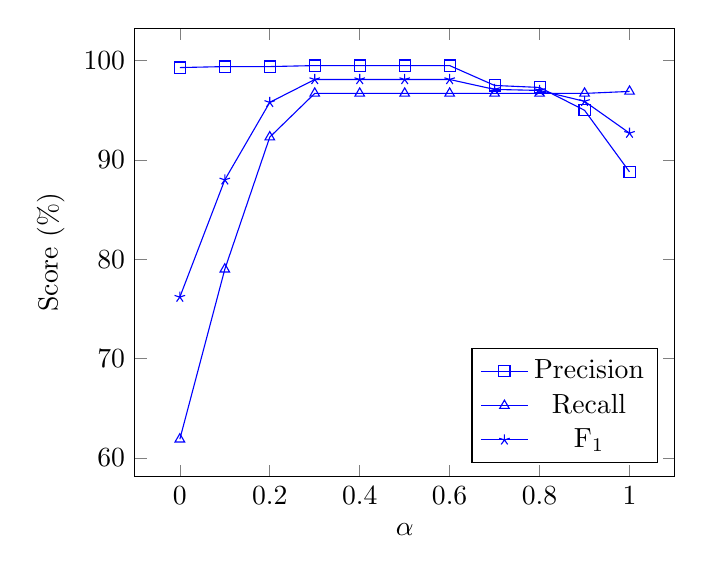
\begin{tikzpicture}
\begin{axis}[xlabel=$\alpha$, ylabel=Score (\%), legend pos=south east]
\addplot[color=blue, mark=square]
coordinates{
  (0, 99.3)(0.1, 99.4)(0.2, 99.4)(0.3, 99.5)(0.4, 99.5)(0.5, 99.5)
  (0.6, 99.5)(0.7, 97.5)(0.8, 97.3)(0.9, 95.0)(1.0, 88.8)
};

\addplot[color=blue, mark=triangle]
coordinates{
  (0, 61.9)(0.1, 79.0)(0.2, 92.3)(0.3, 96.7)(0.4, 96.7)(0.5, 96.7)
  (0.6, 96.7)(0.7, 96.7)(0.8, 96.7)(0.9, 96.7)(1.0, 96.9)
};

\addplot[color=blue, mark=star]
coordinates{
  (0, 76.2)(0.1, 88.0)(0.2, 95.8)(0.3, 98.1)(0.4, 98.1)(0.5, 98.1)
  (0.6, 98.1)(0.7, 97.1)(0.8, 97.0)(0.9, 95.9)(1.0, 92.7)
};

\legend{Precision, Recall, F\textsubscript{1}}
\end{axis}
\end{tikzpicture}
\caption{Precision, Recall和F\textsubscript{1}
随参数$\alpha$的变化情况}
\label{fig:cevc-threshold}
\end{figure}

\subsection{实验结果}
首先对CEVC算法的抽取性能进行实验评估,
表~\ref{tbl:cevc-cevc}~给出了CEVC在新闻和博客数据集上的实验结果,
包含了Precision、Recall、F\textsubscript{1}和Score四项指标。

我们可以看到CEVC算法在30个不同的新闻、博客网站上都取得了良好的内容抽取效果。
对新闻网站的总体抽取效果达到了97.4\%的F\textsubscript{1},
对博客网站的总体抽取效果达到了94.4\%的F\textsubscript{1},
在所有测试集上,F\textsubscript{1}达到了95.8\%。
表明CEVC算法能够适应新闻、博客类网站的核心内容抽取需求。

\begin{table}[htbp]
\caption{CEVC在新闻和博客数据集上的实验结果}
\label{tbl:cevc-cevc}
\vspace{0.5em}\centering\wuhao
\begin{tabular}{lllllll}
\toprule[1.5pt]
网站 & 网址 & 类型 & Precision & Recall & F\textsubscript{1} & Score \\
\midrule[1pt]
环球网 & www.huanqiu.com & news & 91.1\% & 96.4\% & 93.7\% & 88.1\% \\
人民网 & www.people.com.cn & news & 96.2\% & 99.0\% & 97.6\% & 95.3\% \\
凤凰资讯 & news.ifeng.com & news & 99.5\% & 99.9\% & 99.7\% & 99.4\% \\
央视网新闻 & news.cctv.com & news & 93.7\% & 99.9\% & 96.7\% & 93.7\% \\
联合早报 & www.zaobao.com & news & 97.5\% & 99.1\% & 98.3\% & 96.7\% \\
新华网 & www.xinhuanet.com & news & 98.6\% & 99.9\% & 99.2\% & 98.5\% \\
中国信息网 & www.chinanews.com & news & 98.1\% & 99.9\% & 99.0\% & 98.0\% \\
中国军网 & www.81.cn & news & 97.6\% & 100.0\% & 98.8\% & 97.6\% \\
网易新闻 & news.163.com & news & 94.7\% & 98.8\% & 96.7\% & 93.7\% \\
腾讯新闻 & news.qq.com & news & 93.5\% & 99.9\% & 96.6\% & 93.4\% \\
央广网 & www.cnr.cn & news & 97.7\% & 99.5\% & 98.6\% & 97.2\% \\
参考消息 & www.cankaoxiaoxi.com & news & 95.3\% & 95.4\% & 95.3\% & 91.1\% \\
搜狐新闻 & news.sohu.com & news & 97.5\% & 97.8\% & 97.6\% & 95.4\% \\
南方网 & www.southcn.com & news & 91.5\% & 99.3\% & 95.2\% & 90.9\% \\
新浪新闻 & news.sina.com.cn & news & 96.3\% & 100.0\% & 98.1\% & 96.3\% \\
新闻 & - & - & 95.8\% & 99.1\% & 97.4\% & 95.0\% \\
\hline
和讯博客 & blog.hexun.com & blog & 96.4\% & 97.3\% & 96.8\% & 93.9\% \\
瑞丽博客 & blog.rayli.com.cn & blog & 86.6\% & 97.1\% & 91.6\% & 84.5\% \\
凤凰博客 & blog.ifeng.com & blog & 96.9\% & 93.9\% & 95.3\% & 91.1\% \\
中金博客 & blog.cnfol.com & blog & 86.8\% & 89.2\% & 88.0\% & 78.5\% \\
财经网博客 & blog.caijing.com.cn & blog & 96.3\% & 95.9\% & 96.1\% & 92.5\% \\
博客大巴 & www.blogbus.com & blog & 91.8\% & 100.0\% & 95.7\% & 91.8\% \\
新浪博客 & blog.sina.com.cn & blog & 94.3\% & 86.1\% & 90.0\% & 81.9\% \\
博客日报 & www.bokerb.com & blog & 94.3\% & 97.0\% & 95.7\% & 91.7\% \\
科学网博客 & blog.sciencenet.cn & blog & 94.8\% & 95.0\% & 94.9\% & 90.3\% \\
天涯博客 & blog.tianya.cn & blog & 93.8\% & 97.8\% & 95.8\% & 91.9\% \\
博客中国 & www.blogchina.com & blog & 98.4\% & 99.6\% & 99.0\% & 98.0\% \\
搜狐博客 & blog.sohu.com & blog & 94.4\% & 92.4\% & 93.4\% & 87.6\% \\
东方财富博客 & blog.eastmoney.com & blog & 93.3\% & 97.1\% & 95.2\% & 90.8\% \\
网易博客 & blog.163.com & blog & 81.7\% & 92.5\% & 86.7\% & 76.6\% \\
博客网 & www.bokee.com & blog & 93.5\% & 100.0\% & 96.6\% & 93.5\% \\
博客 & - & - & 93.4\% & 95.5\% & 94.4\% & 89.4\% \\
\hline
总体 & - & - & 94.5\% & 97.2\% & 95.8\% & 92.0\% \\
\bottomrule[1.5pt]
\end{tabular}
\end{table}

然后在同样的数据集上分别测试CETR、CETD和CEPR,并和CEVC算法做比较,
如表~\ref{tbl:cevc-all}~所示。
为了节省篇幅,这里只列出了两个综合性指标F\textsubscript{1}和Score,
以F\textsubscript{1}/Score的形式给出。

表~\ref{tbl:cevc-all}~中每一行代表一个网站的测试结果,
粗体标示的是CETR、CETD、CEPR和CEVC四种不同算法
在F\textsubscript{1}和Score指标上的最优者。
在大约三分之二的测试网站上,CEVC算法都能取得最优的内容抽取结果,
CETD和CEPR在剩余三分之一网站上抽取效果最优。
在总体F\textsubscript{1}指标上,CEVC达到95.8\%,和CETD的95.5\%大致相当,
随后是CEPR的92.5\%,大幅度超越了CETR的75.2\%。

\begin{table}[htbp]
\caption{CETR、CETD、CEPR和CEVC的对比结果}
\label{tbl:cevc-all}
\vspace{0.5em}\centering\wuhao
\begin{tabular}{lllll}
\toprule[1.5pt]
网站 & CETR & CETD & CEPR & CEVC \\
\midrule[1pt]
网易新闻 & 68.3\%/51.9\% & 96.9\%/93.9\% & \textbf{97.9\%}/\textbf{95.9\%} & 96.7\%/93.7\% \\
央视网新闻 & 85.3\%/74.4\% & 95.8\%/91.9\% & \textbf{99.1\%}/\textbf{98.3\%} & 96.7\%/93.7\% \\
凤凰资讯 & 53.8\%/36.8\% & 99.5\%/99.1\% & 95.6\%/91.6\% & \textbf{99.7\%}/\textbf{99.4\%} \\
腾讯新闻 & 80.4\%/67.2\% & 96.4\%/93.0\% & \textbf{96.9\%}/\textbf{93.9\%} & 96.6\%/93.4\% \\
新浪新闻 & 81.4\%/68.7\% & \textbf{98.1\%}/96.2\% & 93.6\%/88.0\% & \textbf{98.1\%}/\textbf{96.3\%} \\
搜狐新闻 & 73.7\%/58.3\% & \textbf{98.6\%}/\textbf{97.3\%} & 96.0\%/92.3\% & 97.6\%/95.4\% \\
中国军网 & 89.6\%/81.2\% & 98.6\%/97.3\% & 97.1\%/94.3\% & \textbf{98.8\%}/\textbf{97.6\%} \\
参考消息 & 46.5\%/30.3\% & \textbf{99.8\%}/\textbf{99.7\%} & 92.6\%/86.3\% & 95.3\%/91.1\% \\
中国信息网 & 86.5\%/76.3\% & \textbf{99.0\%}/\textbf{98.1\%} & 98.9\%/97.8\% & \textbf{99.0\%}/98.0\% \\
央广网 & 85.8\%/75.2\% & 98.5\%/97.1\% & 92.0\%/85.2\% & \textbf{98.6\%}/\textbf{97.2\%} \\
环球网 & 79.6\%/66.1\% & 92.1\%/85.3\% & \textbf{97.0\%}/\textbf{94.3\%} & 93.7\%/88.1\% \\
人民网 & 87.8\%/78.3\% & 96.9\%/93.9\% & 89.6\%/81.2\% & \textbf{97.6\%}/\textbf{95.3\%} \\
南方网 & 87.8\%/78.3\% & \textbf{95.5\%}/\textbf{91.4\%} & 93.3\%/87.5\% & 95.2\%/90.9\% \\
新华网 & 97.1\%/94.3\% & \textbf{99.2\%}/\textbf{98.5\%} & 99.0\%/98.0\% & \textbf{99.2\%}/\textbf{98.5\%} \\
联合早报 & 86.5\%/76.3\% & 96.6\%/93.3\% & 91.3\%/84.0\% & \textbf{98.3\%}/\textbf{96.7\%} \\
新闻 & 76.6\%/62.1\% & \textbf{97.4\%}/94.9\% & 95.6\%/91.6\% & \textbf{97.4\%}/\textbf{95.0\%} \\
\hline
网易博客 & 58.3\%/41.2\% & \textbf{97.1\%}/\textbf{94.4\%} & 92.1\%/85.3\% & 86.7\%/76.6\% \\
财经网博客 & 85.5\%/74.7\% & 93.7\%/88.2\% & 94.0\%/88.6\% & \textbf{96.1\%}/\textbf{92.5\%} \\
中金博客 & 59.4\%/42.3\% & 87.0\%/76.9\% & 62.1\%/45.0\% & \textbf{88.0\%}/\textbf{78.5\%} \\
东方财富博客 & 66.5\%/49.8\% & 87.9\%/78.4\% & 92.1\%/85.3\% & \textbf{95.2\%}/\textbf{90.8\%} \\
和讯博客 & 55.6\%/38.5\% & 88.2\%/78.8\% & 82.7\%/70.4\% & \textbf{96.8\%}/\textbf{93.9\%} \\
凤凰博客 & 67.6\%/51.0\% & \textbf{96.4\%}/\textbf{93.1\%} & 89.3\%/80.7\% & 95.3\%/91.1\% \\
瑞丽博客 & 61.4\%/44.3\% & 88.4\%/79.2\% & 88.8\%/79.9\% & \textbf{91.6\%}/\textbf{84.5\%} \\
科学网博客 & 67.6\%/51.0\% & 89.4\%/80.8\% & 91.0\%/83.6\% & \textbf{94.9\%}/\textbf{90.3\%} \\
新浪博客 & 82.4\%/70.1\% & \textbf{90.0\%}/81.8\% & 86.4\%/76.1\% & \textbf{90.0\%}/\textbf{81.9\%} \\
搜狐博客 & 78.5\%/64.7\% & 93.1\%/87.0\% & 86.0\%/75.4\% & \textbf{93.4\%}/\textbf{87.6\%} \\
天涯博客 & 91.0\%/83.5\% & \textbf{98.9\%}/\textbf{97.8\%} & 91.3\%/83.9\% & 95.8\%/91.9\% \\
博客大巴 & 87.1\%/77.2\% & 95.4\%/91.2\% & \textbf{97.1\%}/\textbf{94.4\%} & 95.7\%/91.8\% \\
博客中国 & 90.8\%/83.2\% & 98.3\%/96.7\% & 93.6\%/88.0\% & \textbf{99.0\%}/\textbf{98.0\%} \\
博客网 & 80.8\%/67.8\% & 95.6\%/91.5\% & 86.9\%/76.8\% & \textbf{96.6\%}/\textbf{93.5\%} \\
博客日报 & 85.5\%/74.7\% & \textbf{97.2\%}/\textbf{94.5\%} & 96.5\%/93.2\% & 95.7\%/91.7\% \\
博客 & 73.9\%/58.6\% & 93.8\%/88.2\% & 89.6\%/81.1\% & \textbf{94.4\%}/\textbf{89.4\%} \\
\hline
总体 & 75.2\%/60.2\% & 95.5\%/91.3\% & 92.5\%/86.0\% & \textbf{95.8\%}/\textbf{92.0\%} \\
\bottomrule[1.5pt]
\end{tabular}
\end{table}

虽然新闻、博客类网站结构相近,能够使用同一种内容抽取算法处理,
但从表~\ref{tbl:cevc-all}~中的结果可以看出,
不同算法在博客上的抽取效果都不同程度地低于新闻。
因此有必要对新闻和博客分类计算各项指标,为了更直观地显示,
绘制成表~\ref{fig:cevc-prfs}~所示的折线图,四种算法分别以四种不同的折线表示。

在各项指标上,四种算法抽取博客网站的效果都较新闻网站有不同程度的下降。
CEVC的下降幅度最小,而CEPR和CETR的召回率下降幅度最大,
从对新闻的99\%左右下降到对博客的88\%左右。
CEVC对新闻和博客的抽取效果更为稳定,优于对比算法。

\begin{figure}[htbp]
\centering
\begin{tikzpicture}
\begin{groupplot}[
group style={group size=2 by 2, vertical sep=1.5cm},
legend style={at={(1, 0.7)},anchor=north east},
height=0.4\textwidth,
]

\nextgroupplot[
title=Precision,
symbolic x coords={News, Blog, Average},
xtick=data,
]
\addplot[color=blue, mark=square*, dashed]
coordinates{(News, 62.5) (Blog, 63.7) (Average, 63.1)};
\addplot[color=green, mark=triangle*, dashed]
coordinates{(News, 95.3) (Blog, 93.9) (Average, 94.6)};
\addplot[color=orange, mark=otimes*, thick]
coordinates{(News, 92.7) (Blog, 91.4) (Average, 92.1)};
\addplot[color=red, mark=o, thick]
coordinates{(News, 95.8) (Blog, 93.4) (Average, 94.5)};
\legend{CETR, CETD, CEPR, CEVC}

\nextgroupplot[
title=Recall,
symbolic x coords={News, Blog, Average},
xtick=data,
]
\addplot[color=blue, mark=square*, dashed]
coordinates{(News, 99.0) (Blog, 87.9) (Average, 93.0)};
\addplot[color=green, mark=triangle*, dashed]
coordinates{(News, 99.6) (Blog, 93.6) (Average, 96.4)};
\addplot[color=orange, mark=otimes*, thick]
coordinates{(News, 98.7) (Blog, 87.8) (Average, 92.9)};
\addplot[color=red, mark=o, thick]
coordinates{(News, 99.1) (Blog, 95.5) (Average, 97.2)};


\nextgroupplot[
title=F\textsubscript{1},
symbolic x coords={News, Blog, Average},
xtick=data,
]
\addplot[color=blue, mark=square*, dashed]
coordinates{(News, 76.6) (Blog, 73.9) (Average, 75.2)};
\addplot[color=green, mark=triangle*, dashed]
coordinates{(News, 97.4) (Blog, 93.8) (Average, 95.5)};
\addplot[color=orange, mark=otimes*, thick]
coordinates{(News, 95.6) (Blog, 89.6) (Average, 92.5)};
\addplot[color=red, mark=o, thick]
coordinates{(News, 97.4) (Blog, 94.4) (Average, 95.8)};

\nextgroupplot[
title=Score,
symbolic x coords={News, Blog, Average},
xtick=data,
]
\addplot[color=blue, mark=square*, dashed]
coordinates{(News, 62.1) (Blog, 58.6) (Average, 60.2)};
\addplot[color=green, mark=triangle*, dashed]
coordinates{(News, 94.9) (Blog, 88.2) (Average, 91.3)};
\addplot[color=orange, mark=otimes*, thick]
coordinates{(News, 91.6) (Blog, 81.1) (Average, 86.0)};
\addplot[color=red, mark=o, thick]
coordinates{(News, 95.0) (Blog, 89.4) (Average, 92.0)};

\end{groupplot}
\end{tikzpicture}
\caption{CETR、CETD、CEPR和CEVC在新闻、博客数据集上的各项指标}
\label{fig:cevc-prfs}
\end{figure}

\subsection{结果分析}

相对于职业编辑撰写的新闻,博客的内容由用户编辑产生,形式更加自由,
所使用的HTML标签和样式也更丰富,所以不同方法对博客内容的抽取效果都有所下降。
新闻正文一般由\texttt{<p>}标签组成的段落构成,格式简洁也很扁平化,
而博客内容可以由富文本编辑器产生,带有字体、颜色、大小等控制标签,
结构上层次也比较深,给准确抽取内容带来了挑战。

CETR算法对新闻和博客的整体抽取F\textsubscript{1}只有75.2\%,
虽然召回率93\%较高,但大幅度牺牲了精确率63.1\%。

CETR算法以“行”为单位处理HTML文档,针对每一行计算Tag Ratio,
根据Tag Ratio的高低来划分内容或噪声。
虽然算法经过了平滑处理,也结合序列信息转化为二维数据处理,但从实验结果来看,
依然将一部分噪声标记为内容,例如推荐文章、免责声明等。
CETR对每一行都平等对待,没有结合DOM的结构信息,局部的文本密集也被识别为有效内容,
这就导致最终的结果精确率很低。

CETD算法的整体抽取性能和CEVC基本相当,对新闻的F\textsubscript{1}都是97.4\%,
总体F\textsubscript{1}分别是95.5\%和95.8\%,几乎没有差别。

这是由于两者的核心评估指标相似,CETD基于DOM节点的文本密度,
CEVC基于DOM节点的有效字符数量,也都考虑了链接与网页噪声之间的相关性。
CETD基于DensitySum的方式,选取子节点文本密度之和最大的节点标记为内容,
而CEVC则从\texttt{<body>}开始,逐层选择有效字符最多的子节点不断深入,
二者的输出都是一个特定DOM节点下的文本内容,所以整体抽取效果很接近。

实验早期CETD算法对博客网站的F\textsubscript{1}不足90\%,
分析具体网页后发现,部分博客网站包含\texttt{<textarea>}这样的标签,
标签内部包含大量代码,导致CETD对文本密度的计算向\texttt{<textarea>}倾斜,
最终错误地选择\texttt{<textarea>}作为正文内容。
为了更好地比较CETD算法的性能,在预处理阶段,
除了\texttt{<script>}和\texttt{<style>}之外,还去除了\texttt{<textarea>}标签。
最终的实验结果如表~\ref{tbl:cevc-all}~所示,
对博客网站的F\textsubscript{1}提升到93.8\%。
这表明虽然CETD和CEVC的抽取性能相当,但其预处理阶段需要处理更多的特殊标签,
而CEVC算法加入了对停止词的识别,从而能够有效区分文本内容,不受这些标签的干扰。

CEPR算法的整体F\textsubscript{1}为92.5\%,精确率和召回率都在92\%左右,
对精确率和召回率都没有偏倚。

CEPR的计算过程和CETR有相似之处,CETR以“行”为单位,
而CEPR以路径模式为单位,对每个文本叶节点计算出一个指标。
二者也都进行了高斯平滑,只不过CEPR的平滑过程加入了路径编辑距离的权重。
CEPR的抽取效果较CETR提升很多,但分散的文本叶节点之间,只靠路径模式的相似性关联,
容易被遗漏或误报,不如CETD和CEVC基于DOM内容节点整体来做决策。

CEVC算法对正文内容较短的网页,抽取效果较差。
如表~\ref{tbl:cevc-all}~所示,参考消息和环球网包含部分短讯,
新闻主体内容很短,导致算法错误地将推荐文章、新闻评价板块标记为核心内容,
从而降低了F\textsubscript{1}。
这也是CEVC基于文本聚集程度来划分核心内容的一个缺陷。

以图~\ref{fig:blog-compare}~的一篇
科学网博客\footnote{http://blog.sciencenet.cn/}为例,
直观地比较不同算法的抽取区域。
图中标记了A、B、C、D四个区域,A、B、C为博客正文,而D为博客的相关推荐文章。
\begin{itemize}
\item CETR算法抽取结果为A、B、C、D,虽然没有遗漏正文,却包含了噪声部分D。
\item CETD算法抽取结果为B,这是因为B区域是一个\texttt{<backquote>}标签,
包含了许多\texttt{<p>}标签,其子节点的文本密度之和最大,从而遗漏了A和C。
\item CEPR算法根据路径模式划分内容,丢弃了Tag Path Ratio较低的A部分,选择了B和C。
\item CEVC算法根据有效字符在DOM树中的分布,正确地选择了A、B、C作为核心内容。
\end{itemize}

\begin{figure}[htbp]
\centering
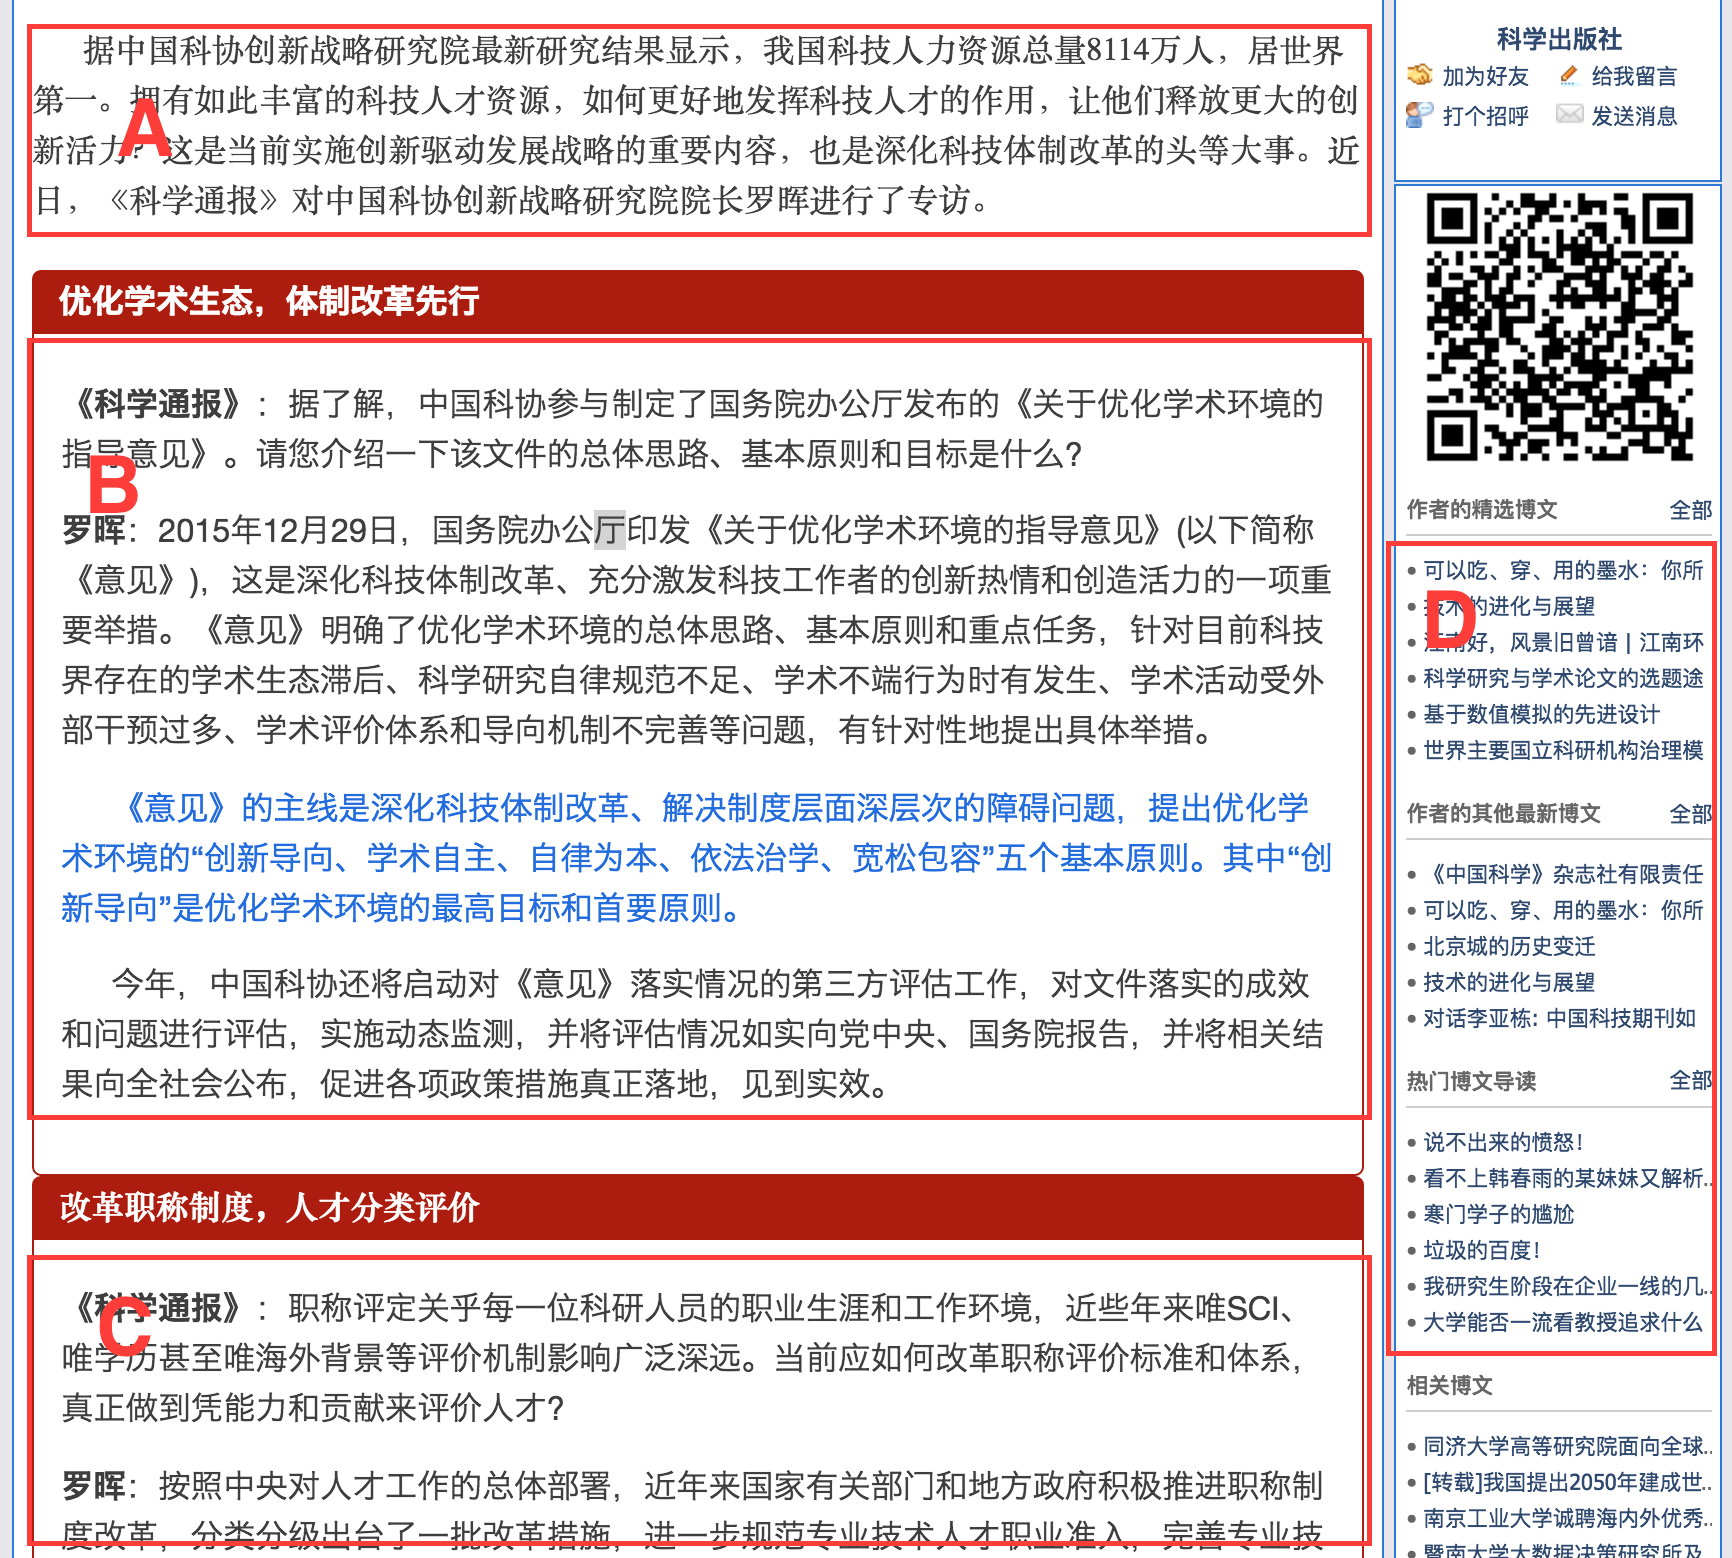
\includegraphics[width=0.9\textwidth,height=0.45\textheight]{blog-compare}
\caption{不同算法的抽取区域比较}
\label{fig:blog-compare}
\end{figure}
